\begin{dang}{Biểu diễn góc trên đường tròn lượng giác}
	Để biểu diễn các góc lượng giác trên đường tròn lượng giác ta thường sử dụng các kết quả sau:
	\begin{itemize}
		\item Góc $\alpha\ \left(a^{\circ}\right)$  và cung có số đo $\alpha+k 2 \pi, k \in \mathbb{Z}\ \left(a^{\circ}+k360^{\circ}\right)$ có cùng điểm biểu diễn trên đường tròn lượng giác.
		\item Số điểm trên đường tròn lượng giác biểu diễn góc lượng giác số đo có dạng $\alpha+\dfrac{k 2 \pi}{m}\ \left(\text{hay } a^{\circ}+\dfrac{k360^{\circ}}{m}\right)$ (với $k$ là số nguyên và $m$ là số nguyên dương) là $m$. Từ đó để biểu diễn các góc lượng giác đó ta lần lượt cho $k$ từ 0 tới $m-1$ rồi biểu diễn các góc đó.
	\end{itemize}
	
\end{dang}
\subsubsection{Ví dụ minh hoạ}
\begin{vd} %[1K1B1-4]
	Biểu diễn trên đường tròn lượng giác các góc lượng giác có số đo là 
	\begin{enumEX}{4}
		\item $865^{\circ}$;
		\item $-1485^{\circ}$;
		\item $\dfrac{13}{3}\pi$;
		\item $-\dfrac{7}{3}\pi$.
	\end{enumEX}
	\loigiai{
	\begin{enumerate}
	\item Ta có $865^{\circ}=145^{\circ}+2\cdot360^{\circ}$. Vậy điểm biểu diễn góc lượng giác có số đo $865^{\circ}$ là điểm $M$ trên phần đường tròn lượng giác thuộc góc phần tư thứ II sao cho $\widehat{A O M}=145^{\circ}$. 
	\begin{center}
		\begin{tikzpicture}[scale=.8,>=stealth, font=\footnotesize, line join=round, line cap=round]
			\draw[fill=black](0,0) coordinate (O) node[below left]{$O$} circle (1.5pt) (2,0) coordinate (A) node[above right] {$A$} circle (1.5pt) (145:2) coordinate (M) node [left] {$M$} circle (1.5 pt);
			\draw[very thick] (0,0) circle (2 cm);
			\draw[->] (-3,0)--(3,0) node [below]{$x$};
			\draw[->] (0,-3)--(0,3) node [left]{$y$};
			\clip (-5,-5) rectangle (5,5);
			\draw (3,3) node {I} (-3,3) node {II} (-3,-3) node {III} (3,-3) node {IV};
			\draw (M)--(O);
			\pic [draw, ->, "$\alpha$", angle eccentricity=1.5] {angle = A--O--M};
		\end{tikzpicture}
	\end{center}
	\item Ta có $-1485^{\circ}=-45^{\circ}-3\cdot360^{\circ}$. Vậy điểm biểu diễn góc lượng giác có số đo $-1485^{\circ}$ là điểm $M$ trên phần đường tròn lượng giác thuộc góc phần tư thứ IV sao cho  $\widehat{A O M}=145^{\circ}$.
	\begin{center}
		\begin{tikzpicture}[scale=.8,>=stealth, font=\footnotesize, line join=round, line cap=round]
			\draw[fill=black](0,0) coordinate (O) node[below left]{$O$} circle (1.5pt) (2,0) coordinate (A) node[above right] {$A$} circle (1.5pt) (-45:2) coordinate (M) node [below right] {$M$} circle (1.5 pt);
			\draw[very thick] (0,0) circle (2 cm);
			\draw[->] (-3,0)--(3,0) node [below]{$x$};
			\draw[->] (0,-3)--(0,3) node [left]{$y$};
			\clip (-5,-5) rectangle (5,5);
			\draw (3,3) node {I} (-3,3) node {II} (-3,-3) node {III} (3,-3) node {IV};
			\draw (M)--(O);
			\pic [draw, <-, "$\alpha$", angle eccentricity=1.5] {angle = M--O--A};
		\end{tikzpicture}
	\end{center}
	\item Ta có $\dfrac{13}{3}\pi=\dfrac{\pi}{3}+2\cdot2\pi$. Vậy điểm biểu diễn góc lượng giác có số đo $\dfrac{13}{3}\pi$ là điểm $M$ trên phần đường tròn lượng giác thuộc góc phần tư thứ I sao cho $\widehat{A O M}=\dfrac{\pi}{3}$. 
	\begin{center}
		\begin{tikzpicture}[scale=.8,>=stealth, font=\footnotesize, line join=round, line cap=round]
			\draw[fill=black](0,0) coordinate (O) node[below left]{$O$} circle (1.5pt) (2,0) coordinate (A) node[above right] {$A$} circle (1.5pt) (60:2) coordinate (M) node [above right] {$M$} circle (1.5 pt);
			\draw[very thick] (0,0) circle (2 cm);
			\draw[->] (-3,0)--(3,0) node [below]{$x$};
			\draw[->] (0,-3)--(0,3) node [left]{$y$};
			\clip (-5,-5) rectangle (5,5);
			\draw (3,3) node {I} (-3,3) node {II} (-3,-3) node {III} (3,-3) node {IV};
			\draw (M)--(O);
			\pic [draw, ->, "$\alpha$", angle eccentricity=1.5] {angle = A--O--M};
		\end{tikzpicture}
	\end{center}
	\item Ta có $-\dfrac{7}{3}\pi=-\dfrac{\pi}{3}-2\pi$. Vậy điểm biểu diễn góc lượng giác có số đo $-\dfrac{7}{3}\pi$ là điểm $M$ trên phần đường tròn lượng giác thuộc góc phần tư thứ IV sao cho $\widehat{A O M}=\dfrac{\pi}{3}$. 
	\begin{center}
		\begin{tikzpicture}[scale=.8,>=stealth, font=\footnotesize, line join=round, line cap=round]
			\draw[fill=black](0,0) coordinate (O) node[below left]{$O$} circle (1.5pt) (2,0) coordinate (A) node[above right] {$A$} circle (1.5pt) (-60:2) coordinate (M) node [below right] {$M$} circle (1.5 pt);
			\draw[very thick] (0,0) circle (2 cm);
			\draw[->] (-3,0)--(3,0) node [below]{$x$};
			\draw[->] (0,-3)--(0,3) node [left]{$y$};
			\clip (-5,-5) rectangle (5,5);
			\draw (3,3) node {I} (-3,3) node {II} (-3,-3) node {III} (3,-3) node {IV};
			\draw (M)--(O);
			\pic [draw, <-, "$\alpha$", angle eccentricity=1.5] {angle = M--O--A};
		\end{tikzpicture}
	\end{center}
	\end{enumerate}

}
\end{vd}
\begin{vd} %[1K1K1-4]
	Biểu diễn trên đường tròn lượng giác các góc lượng giác có số đo sau (với $k$ là số nguyên tùy ý)
	\begin{enumEX}{2}
		\item $\alpha=k\pi$;
		\item $\alpha=\dfrac{\pi}{3}+k\pi$.
	\end{enumEX}
\loigiai{\immini{
	\begin{enumerate}
		\item Ta có $\alpha=k\pi=\dfrac{k2\pi}{2}$ do đó có hai điểm biểu diễn bởi góc có số đo $\alpha$.\\
		Với $k=0$, ta có $\alpha=0$ được biểu diễn bởi điểm $A_1$.\\
		Với $k=1$, ta có $\alpha=\pi$ được biểu diễn bởi điểm $A_2$.
		\item Ta có $\alpha=\dfrac{\pi}{3}+k\pi=\dfrac{\pi}{3}+\dfrac{k2\pi}{2}$ do đó có hai điểm biểu diễn bởi góc có số đo $\alpha$.\\
		Với $k=0$, ta có $\alpha=\dfrac{\pi}{3}$ được biểu diễn bởi điểm $B_1$.\\
		Với $k=1$, ta có $\alpha=\dfrac{4\pi}{3}$ được biểu diễn bởi điểm $B_2$.
	\end{enumerate}
}{
		\begin{tikzpicture}[scale=.8,>=stealth, font=\footnotesize, line join=round, line cap=round]
			\draw[fill=black](0,0) coordinate (O) node[below left]{$O$} circle (1.5pt) (2,0) coordinate (A) node[above right] {$A_1$} circle (1.5pt) (180:2) coordinate (A2) node [above left] {$A_2$} circle (1.5 pt) (60:2) coordinate (B1) node [above right] {$B_1$} circle (1.5pt) (240:2) coordinate (B2) node [below left] {$B_2$} circle (1.5pt);
			\draw[very thick] (0,0) circle (2 cm);
			\draw[->] (-3,0)--(3,0) node [below]{$x$};
			\draw[->] (0,-3)--(0,3) node [left]{$y$};
			\clip (-5,-5) rectangle (5,5);
		\end{tikzpicture}
}
}
\end{vd}
\subsubsection{Bài tập vận dụng}
\begin{bt}%[1K1B1-4]
	Biểu diễn trên đường tròn lượng giác các góc lượng giác có số đo sau:
	\begin{enumEX}{2}
		\item $750^{\circ}$;
		\item $-1125^{\circ}$.
	\end{enumEX}
\loigiai{
	\begin{enumerate}
		\item Ta có $750^{\circ}=30^{\circ}+2\cdot360^{\circ}$. Vậy điểm biểu diễn góc lượng giác có số đo $750^{\circ}$ là điểm $M$ trên phần đường tròn lượng giác thuộc góc phần tư thứ I sao cho $\widehat{A O M}=30^{\circ}$. 
		\begin{center}
			\begin{tikzpicture}[scale=.8,>=stealth, font=\footnotesize, line join=round, line cap=round]
				\draw[fill=black](0,0) coordinate (O) node[below left]{$O$} circle (1.5pt) (2,0) coordinate (A) node[above right] {$A$} circle (1.5pt) (30:2) coordinate (M) node [right] {$M$} circle (1.5 pt);
				\draw[very thick] (0,0) circle (2 cm);
				\draw[->] (-3,0)--(3,0) node [below]{$x$};
				\draw[->] (0,-3)--(0,3) node [left]{$y$};
				\clip (-5,-5) rectangle (5,5);
				\draw (3,3) node {I} (-3,3) node {II} (-3,-3) node {III} (3,-3) node {IV};
				\draw (M)--(O);
				\pic [draw, ->, "$\alpha$", angle eccentricity=1.5] {angle = A--O--M};
			\end{tikzpicture}
		\end{center}
		\item Ta có $-1125^{\circ}=-45^{\circ}-3\cdot360^{\circ}$. Vậy điểm biểu diễn góc lượng giác có số đo $-1125^{\circ}$ là điểm $M$ trên phần đường tròn lượng giác thuộc góc phần tư thứ IV sao cho $\widehat{A O M}=45^{\circ}$. 
		\begin{center}
			\begin{tikzpicture}[scale=.8,>=stealth, font=\footnotesize, line join=round, line cap=round]
				\draw[fill=black](0,0) coordinate (O) node[below left]{$O$} circle (1.5pt) (2,0) coordinate (A) node[above right] {$A$} circle (1.5pt) (-45:2) coordinate (M) node [below right] {$M$} circle (1.5 pt);
				\draw[very thick] (0,0) circle (2 cm);
				\draw[->] (-3,0)--(3,0) node [below]{$x$};
				\draw[->] (0,-3)--(0,3) node [left]{$y$};
				\clip (-5,-5) rectangle (5,5);
				\draw (3,3) node {I} (-3,3) node {II} (-3,-3) node {III} (3,-3) node {IV};
				\draw (M)--(O);
				\pic [draw, <-, "$\alpha$", angle eccentricity=1.5] {angle = M--O--A};
			\end{tikzpicture}
		\end{center}
	\end{enumerate}
}
\end{bt}
\begin{bt}%[1K1B1-4]
	Biểu diễn trên đường tròn lượng giác các góc lượng giác có số đo sau:
	\begin{enumEX}{2}
		\item $\dfrac{9\pi}{2}$;
		\item $-\dfrac{37\pi}{6}$.
	\end{enumEX}
\loigiai{
	\begin{enumerate}
	\item Ta có $\dfrac{9\pi}{2}=\dfrac{\pi}{2}+2\cdot2\pi$. Vậy điểm biểu diễn góc lượng giác có số đo $\dfrac{9\pi}{2}$ là điểm $M$ trên phần đường tròn lượng giác sao cho $\widehat{A O M}=\dfrac{\pi}{2}$. 
	\begin{center}
		\begin{tikzpicture}[scale=.8,>=stealth, font=\footnotesize, line join=round, line cap=round]
			\draw[fill=black](0,0) coordinate (O) node[below left]{$O$} circle (1.5pt) (2,0) coordinate (A) node[above right] {$A$} circle (1.5pt) (90:2) coordinate (M) node [above right] {$M$} circle (1.5 pt);
			\draw[very thick] (0,0) circle (2 cm);
			\draw[->] (-3,0)--(3,0) node [below]{$x$};
			\draw[->] (0,-3)--(0,3) node [left]{$y$};
			\clip (-5,-5) rectangle (5,5);
			\draw (3,3) node {I} (-3,3) node {II} (-3,-3) node {III} (3,-3) node {IV};
			\draw (M)--(O);
			\pic [draw, ->, "$\alpha$", angle eccentricity=1.5] {angle = A--O--M};
		\end{tikzpicture}
	\end{center}
	\item Ta có $-\dfrac{37\pi}{6}=-\dfrac{\pi}{6}-3\cdot2\pi$. Vậy điểm biểu diễn góc lượng giác có số đo $-\dfrac{37\pi}{6}$ là điểm $M$ trên phần đường tròn lượng giác thuộc góc phần tư thứ IV sao cho $\widehat{A O M}=\dfrac{\pi}{6}$. 
	\begin{center}
		\begin{tikzpicture}[scale=.8,>=stealth, font=\footnotesize, line join=round, line cap=round]
			\draw[fill=black](0,0) coordinate (O) node[below left]{$O$} circle (1.5pt) (2,0) coordinate (A) node[above right] {$A$} circle (1.5pt) (-30:2) coordinate (M) node [below right] {$M$} circle (1.5 pt);
			\draw[very thick] (0,0) circle (2 cm);
			\draw[->] (-3,0)--(3,0) node [below]{$x$};
			\draw[->] (0,-3)--(0,3) node [left]{$y$};
			\clip (-5,-5) rectangle (5,5);
			\draw (3,3) node {I} (-3,3) node {II} (-3,-3) node {III} (3,-3) node {IV};
			\draw (M)--(O);
			\pic [draw, <-, "$\alpha$", angle eccentricity=1.5] {angle = M--O--A};
		\end{tikzpicture}
	\end{center}
	\end{enumerate}
}
\end{bt}
\begin{bt}%[1K1K1-4]
	Biểu diễn trên đường tròn lượng giác các góc lượng giác có số đo sau:
	\begin{enumEX}{2}
		\item $\dfrac{\pi}{6}+k\pi$;
		\item $-\dfrac{\pi}{4}+\dfrac{k2\pi}{3}$.
	\end{enumEX}
	\loigiai{
\immini{
	\begin{enumerate}
		\item Ta có $\alpha=\dfrac{\pi}{6}+k\pi=\dfrac{\pi}{6}+\dfrac{k2\pi}{2}$ do đó có hai điểm biểu diễn góc  $\alpha$ lần lượt là $\dfrac{\pi}{6}$ biểu diễn bởi $A_1$ và $\dfrac{7\pi}{6}$ biểu diễn $A_2$.
		\item Ta có $\alpha=\dfrac{\pi}{4}+\dfrac{k2\pi}{3}$ có ba điểm biểu diễn góc $\alpha$ lần lượt là $\dfrac{\pi}{4}$ biểu diễn bởi $B_1$, $\dfrac{11\pi}{12}$ biểu diễn bởi $B_2$ và $\dfrac{19\pi}{12}$ biểu diễn bởi $B_3$.
	\end{enumerate}
}{
	\begin{tikzpicture}[scale=.8,>=stealth, font=\footnotesize, line join=round, line cap=round]
		\draw[fill=black](0,0) coordinate (O) node[below left]{$O$} circle (1.5pt) (30:2) coordinate (A1) node[right] {$A_1$} circle (1.5pt) (210:2) coordinate (A2) node [below left] {$A_2$} circle (1.5 pt) (45:2) coordinate (B1) node [above right] {$B_1$} circle (1.5pt) (165:2) coordinate (B2) node [above left] {$B_2$} circle (1.5pt) (285:2) coordinate (B3) node [below right] {$B_3$} circle (1.5pt);
		\draw[very thick] (0,0) circle (2 cm);
		\draw[->] (-3,0)--(3,0) node [below]{$x$};
		\draw[->] (0,-3)--(0,3) node [left]{$y$};
		\clip (-5,-5) rectangle (5,5);
	\end{tikzpicture}
}
}
\end{bt}
\begin{bt}%[1K1K1-4]
	Khi biểu diễn các góc lượng giác có số đo $x=\dfrac{\pi}{2}+k \pi$ và $y=\dfrac{\pi}{2}+k 2 \pi$ lên đường tròn lượng giác, số điểm chung nhận được là bao nhiêu?
	\loigiai{
	Ta có $x=\dfrac{\pi}{2}+k \pi=\dfrac{\pi}{2}+\dfrac{k 2 \pi}{2}$. Vậy có 2 điểm biểu diễn góc lượng giác có số đo $x$.
	\begin{itemize}
	\item 	Với $k=0,\ x_1=\dfrac{\pi}{2}$, được biểu diễn bởi điểm $B$.
	\item 	Với $k=1,\ x_2=\dfrac{3 \pi}{2}$ được biểu diễn bởi điểm $B'$.
	\end{itemize}
	Ta có $y=\dfrac{\pi}{2}+k 2 \pi$. Vậy có 1 điểm biểu diễn góc lượng giác có số đo $y$. Với $k=0, y=\dfrac{\pi}{2}$, được biểu diễn bởi điểm $B$. Vậy số điểm chung nhận được là 1 điểm chung.
}
\end{bt}
\begin{bt}%[1K1G1-4]
	Xác định công thức hợp nhất của hai góc lượng giác $x_1=k\pi$ và $x_2=\dfrac{\pi}{2}+k\pi$.
	\loigiai{
	Ta có $x_1=k\pi=\dfrac{k2\pi}{2}$ có hai điểm biểu diễn cho góc $x_1$ với $0$ biểu diễn bởi $A_1$ và $\pi$ biểu diễn bởi $A_2$.\\
	$x_2 = \dfrac{\pi}{2}+k\pi=\dfrac{\pi}{2}+\dfrac{k2\pi}{2}$ có hai điểm biểu diễn với $\dfrac{\pi}{2}$ biểu diễn bởi $B_1$ và $\dfrac{3\pi}{2}$ biểu diễn bởi $B_2$.\\
	Dễ thấy 4 điểm này cách đều nhau do đó có thể gộp hai hai góc lượng giác này lại thành công thức duy nhất là $\dfrac{k2\pi}{4}=\dfrac{k\pi}{2}$. 
}
\end{bt}
\subsubsection{Bài tập trắc nghiệm}
\Opensolutionfile{ans}[ans/ans-1K1-1-Dang4]
\begin{ex}%[1K1Y1-4]
	Góc lượng giác $\dfrac{31 \pi}{7}$ có cùng điểm biểu diễn trên đường tròn lượng giác với góc lượng giác nào sau đây?
	\choice
	{\True$\dfrac{3 \pi}{7}$}
	{$\dfrac{10 \pi}{7}$}
	{$\dfrac{-25 \pi}{7}$}
	{$\dfrac{2\pi}{5}$}
	\loigiai{
	Ta có $\dfrac{31\pi}{7}=\dfrac{3\pi}{7}+2\cdot 2\pi$, do đó góc lượng giác $\dfrac{31\pi}{7}$ có cùng điểm biểu diễn với góc $\dfrac{3\pi}{7}$.
	}
\end{ex}
\begin{ex}%[1K1Y1-4]
	Các góc lượng giác nào sau đây có cùng điểm biểu diễn trên đường tròn lượng giác?
	\choice
	{$45^{\circ}$; $405^{\circ}$; $750^{\circ}$}
	{$30^{\circ}$; $405^{\circ}$; $750^{\circ}$}
	{$60^{\circ}$; $405^{\circ}$; $750^{\circ}$}
	{\True $45^{\circ}$; $405^{\circ}$; $765^{\circ}$}
	\loigiai{
	Ta có $405^{\circ}=45^{\circ}+360^{\circ}$ và $765^{\circ}=45^{\circ}+2\cdot360^{\circ}$.\\
	Do đó $45^{\circ}$; $405^{\circ}$; $765^{\circ}$ có cùng điểm biểu diễn trên đường tròn lượng giác.
	}
\end{ex}
\begin{ex}%[1K1Y1-4]
	\immini{
	Hình vẽ bên dưới biểu diễn cho góc lượng giác nào sau đây?
	\choice
	{$30^{\circ}$}
	{$90^{\circ}$}
	{\True $125^{\circ}$}
	{$-60^{\circ}$}
	}{\begin{tikzpicture}[scale=.6,>=stealth, font=\footnotesize, line join=round, line cap=round]
		\draw[fill=black](0,0) coordinate (O) node[below left]{$O$} circle (1.5pt) (2,0) coordinate (A) node[above right] {$A$} circle (1.5pt) (125:2) coordinate (M) node [above left] {$M$} circle (1.5 pt);
		\draw[very thick] (0,0) circle (2 cm);
		\draw[->] (-3,0)--(3,0) node [below]{$x$};
		\draw[->] (0,-3)--(0,3) node [left]{$y$};
		\clip (-5,-5) rectangle (5,5);
		\draw (3,3) node {I} (-3,3) node {II} (-3,-3) node {III} (3,-3) node {IV};
		\draw (M)--(O);
		\pic [draw, ->, "$\alpha$", angle eccentricity=1.5] {angle = A--O--M};
	\end{tikzpicture}}
	\loigiai{
		
	}
\end{ex}
\begin{ex}%[1K1Y1-4]
	Điểm $M$ biểu diễn góc lượng giác có số đo $\alpha=-765^{\circ}$ nằm ở góc phần tư nào?
	\choice
	{Góc phần tư thứ I}
	{Góc phần tư thứ II}
	{Góc phần tư thứ III}
	{\True Góc phần tư thứ IV}

	% \choice
	% {\begin{tikzpicture}[scale=.4,>=stealth, font=\footnotesize, line join=round, line cap=round]
	% 		\draw[fill=black](0,0) coordinate (O) node[below left]{$O$} circle (1.5pt) (2,0) coordinate (A) node[above right] {$A$} circle (1.5pt) (145:2) coordinate (M) node [left] {$M$} circle (1.5 pt);
	% 		\draw[very thick] (0,0) circle (2 cm);
	% 		\draw[->] (-3,0)--(3,0) node [below]{$x$};
	% 		\draw[->] (0,-3)--(0,3) node [left]{$y$};
	% 		\clip (-5,-5) rectangle (5,5);
	% 		\draw (3,3) node {I} (-3,3) node {II} (-3,-3) node {III} (3,-3) node {IV};
	% 		\draw (M)--(O);
	% 		% \pic [draw, ->, "$\alpha$", angle eccentricity=1.5] {angle = A--O--M};
	% \end{tikzpicture}}
	% {\True \begin{tikzpicture}[scale=.4,>=stealth, font=\footnotesize, line join=round, line cap=round]
	% 		\draw[fill=black](0,0) coordinate (O) node[below left]{$O$} circle (1.5pt) (2,0) coordinate (A) node[above right] {$A$} circle (1.5pt) (-45:2) coordinate (M) node [below right] {$M$} circle (1.5 pt);
	% 		\draw[very thick] (0,0) circle (2 cm);
	% 		\draw[->] (-3,0)--(3,0) node [below]{$x$};
	% 		\draw[->] (0,-3)--(0,3) node [left]{$y$};
	% 		\clip (-5,-5) rectangle (5,5);
	% 		\draw (3,3) node {I} (-3,3) node {II} (-3,-3) node {III} (3,-3) node {IV};
	% 		\draw (M)--(O);
	% 		% \pic [draw, <-, "$\alpha$", angle eccentricity=1.5] {angle = M--O--A};
	% \end{tikzpicture}}
	% {\begin{tikzpicture}[scale=.4,>=stealth, font=\footnotesize, line join=round, line cap=round]
	% 		\draw[fill=black](0,0) coordinate (O) node[below left]{$O$} circle (1.5pt) (2,0) coordinate (A) node[above right] {$A$} circle (1.5pt) (60:2) coordinate (M) node [above right] {$M$} circle (1.5 pt);
	% 		\draw[very thick] (0,0) circle (2 cm);
	% 		\draw[->] (-3,0)--(3,0) node [below]{$x$};
	% 		\draw[->] (0,-3)--(0,3) node [left]{$y$};
	% 		\clip (-5,-5) rectangle (5,5);
	% 		\draw (3,3) node {I} (-3,3) node {II} (-3,-3) node {III} (3,-3) node {IV};
	% 		\draw (M)--(O);
	% 		% \pic [draw, ->, "$\alpha$", angle eccentricity=1.5] {angle = A--O--M};
	% \end{tikzpicture}}
	% {\begin{tikzpicture}[scale=.4,>=stealth, font=\footnotesize, line join=round, line cap=round]
	% 		\draw[fill=black](0,0) coordinate (O) node[below left]{$O$} circle (1.5pt) (2,0) coordinate (A) node[above right] {$A$} circle (1.5pt) (-60:2) coordinate (M) node [below right] {$M$} circle (1.5 pt);
	% 		\draw[very thick] (0,0) circle (2 cm);
	% 		\draw[->] (-3,0)--(3,0) node [below]{$x$};
	% 		\draw[->] (0,-3)--(0,3) node [left]{$y$};
	% 		\clip (-5,-5) rectangle (5,5);
	% 		\draw (3,3) node {I} (-3,3) node {II} (-3,-3) node {III} (3,-3) node {IV};
	% 		\draw (M)--(O);
	% 		% \pic [draw, <-, "$\alpha$", angle eccentricity=1.5] {angle = M--O--A};
	% \end{tikzpicture}}
	\loigiai{
	Ta có $-765^{\circ}=-45^{\circ}-2\cdot 360^{\circ}$. Do đó góc $-765^{\circ}$ có điểm biểu diễn tại vị trí góc phần tư thứ IV và góc $\widehat{AOM}=45^{\circ}$.	
	}
\end{ex}
\begin{ex}%[1K1B1-4]
	Có bao nhiêu điểm trên đường tròn lượng giác biểu diễn cho góc lượng giác $x=\dfrac{\pi}{3}+\dfrac{k\pi}{2}$?
	\choice
	{$1$}
	{$2$}
	{$3$}
	{\True $4$}
	\loigiai{
	Ta có $x=\dfrac{\pi}{3}+\dfrac{k\pi}{2}=\dfrac{\pi}{3}+\dfrac{2k\pi}{4}$. Do đó có 4 diểm biểu diễn cho góc $x$.	
	}
\end{ex}
% \begin{ex}%[1K1B1-4]
% 	Hình vẽ bên dưới biểu diễn cho góc lượng giác nào sau đây?
% 	\begin{center}
% 		\begin{tikzpicture}[scale=.6,>=stealth, font=\footnotesize, line join=round, line cap=round]
% 			\draw[fill=black](0,0) coordinate (O) node[below left]{$O$} circle (1.5pt) (2,0) coordinate (A) node[above right] {$A$} circle (1.5pt) (60:2) coordinate (M) node [above right] {$M$} circle (1.5 pt) (240:2) coordinate (N) node [below left] {$N$} circle (1.5 pt);
% 			\draw[very thick] (0,0) circle (2 cm);
% 			\draw[->] (-3,0)--(3,0) node [below]{$x$};
% 			\draw[->] (0,-3)--(0,3) node [left]{$y$};
% 			\clip (-5,-5) rectangle (5,5);
% %			\draw (3,3) node {I} (-3,3) node {II} (-3,-3) node {III} (3,-3) node {IV};
% 			\draw (M)--(O);
% 			\pic [draw, ->, "$\dfrac{\pi}{3}$", angle eccentricity=1.5] {angle = A--O--M};
% 		\end{tikzpicture}
% 	\end{center}
% 	\choice
% 	{$\dfrac{\pi}{3}$}
% 	{$\dfrac{\pi}{3}+k2\pi$}
% 	{\True $\dfrac{\pi}{3}+k\pi$}
% 	{$\dfrac{\pi}{3}+\dfrac{k\pi}{2}$}
% 	\loigiai{
% 		Ta thấy $\widehat{AOM}=\dfrac{\pi}{3}$ và có hai điểm $M,N$ đối xứng nhau qua $O$ biểu diễn cho góc lượng giác $\alpha$. Do đó, $\alpha$ có thể viết dưới dạng $\dfrac{\pi}{3}+\dfrac{k2\pi}{2}=\dfrac{\pi}{3}+k\pi$. 
% 	}
% \end{ex}

\begin{ex}%[1K1B1-4]
	 Trên đường tròn lượng giác với điểm gốc là $A$. Điểm $M$ thuộc đường tròn sao cho $\widehat{AOM}=75^{\circ}$. Gọi $N$ là điểm đối xứng với điểm $M$ qua gốc tọa độ $O$, số đo góc lượng giác $\widehat{AON}$ bằng
	\choice
	{$255^{\circ}$}
	{$-105^{\circ}$}
	{\True $-105^{\circ}$ hoặc $255^{\circ}$}
	{$-105^{\circ}+k 360^{\circ}, k \in \mathbb{Z}$}
	\loigiai{
	Vì $N$ đối xứng với $M$ qua gốc tọa độ $O$. Do đó $\widehat{AON}=\widehat{AOM}\pm180^{\circ}$, suy ra $\widehat{AON}=255^{\circ}$ hoặc $\widehat{AON}=-105^{\circ}$.
	}
\end{ex}
\begin{ex}%[1K1K1-4]
	Trên đường tròn lượng giác gốc $A$, cung lượng giác nào có các điểm biểu diễn tạo thành hình vuông?
	\choice
	{\True $\dfrac{k \pi}{2}$}
	{$k \pi$}
	{$\dfrac{k 2 \pi}{3}$}
	{$\dfrac{k \pi}{3}$}
	\loigiai{
Ta có $\alpha =\dfrac{k\pi}{2}=\dfrac{k2\pi}{4}$. Do đó có 4 điểm biểu diễn cho góc $\alpha$ và 4 điểm này tạo thành hình vuông trên đường tròn lượng giác.	
	}
\end{ex}

\begin{ex}%[1K1K1-4]
	Cho góc lượng giác có số đo $x=\dfrac{\pi}{4}+k \pi$ với $k$ là số nguyên tùy ý. Có bao nhiêu giá trị $k$ thỏa mãn $x \in[2 \pi; 5 \pi]$?
	\choice
	{$1$}
	{$2$}
	{\True $3$}
	{$4$}
	\loigiai{
	Giải hệ bất phương trình $\heva{&\dfrac{\pi}{4}+k \pi>2 \pi \\& \dfrac{\pi}{4}+k \pi<5} \Leftrightarrow\heva{&k>\dfrac{7}{4} \\& k<\dfrac{19}{4}.}$\\
	Từ đó, để $x \in[2 \pi; 5 \pi]$ thì $\dfrac{7}{4}<k<\dfrac{19}{4}$. \\
	Vì $k$ là số nguyên nên có 3 giá trị của $k$, là $2,3,4$, thỏa mãn ycbt.	
	}
\end{ex}
\begin{ex}%[1K1G1-4]
	\immini[thm]{Hình vẽ bên dưới biểu diễn cánh quạt của động cơ máy bay. Các vị trí $B,C,D$ trên cánh quạt có thể biểu diễn cho góc lượng giác nào sau đây?
	\choice
	{$\dfrac{\pi}{4}+2\pi$}
	{$\dfrac{\pi}{2}+k\pi$}
	{\True$\dfrac{\pi}{2}+\dfrac{k2\pi}{3}$}
	{$\dfrac{-\pi}{4}+\dfrac{k2\pi}{3}$}
	}{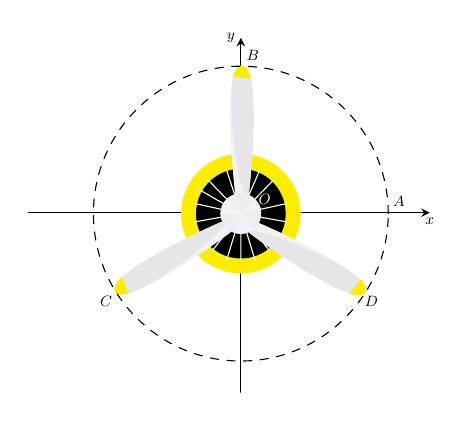
\begin{tikzpicture}[line join=round, line cap=round,scale=0.6,transform shape,>=stealth,font=\small]
		%\draw[gray!50] (-4,-4) grid (4,4);
		\definecolor{aureolin}{rgb}{0.99, 0.93, 0.0}
		\definecolor{anti-flashwhite}{rgb}{0.95, 0.95, 0.96}
		\definecolor{azure(web)(azuremist)}{rgb}{0.94, 1.0, 1.0}
		\def\xmin{-4.5} \def\xmax{4}
		\def\ymin{-4.5} \def\ymax{3} 	
		\draw[->] (\xmin,-.7)--(\xmax,-.7) node [below]{$x$};
		\draw[->] (0,\ymin)--(0,\ymax) node [left]{$y$};
		
		\node at (0,2.4) [above right]{$B$};
		\node at (3.1,-.7) [above right]{$A$};
		\node at (2.5,-2.8) [above right]{$D$};
		\node at (-2.6,-2.8) [above left]{$C$};
		\clip (\xmin+0.1,\ymin+0.1) rectangle (\xmax-0.1,\ymax-0.1);
		
		\tikzset{canh/.pic={
				\def\B{ 
					(-.1,-.35)
					..controls +(100:.2) and +(140:.7) ..(.1,2.35)
					..controls +(-40:.4) and +(80:.2) ..(.15,-.35)
					..controls +(160:.1) and +(20:.1) ..cycle
					;}
				\draw[anti-flashwhite]\B;
				\fill[anti-flashwhite] \B;
				
				\def\A{ 
					(.15,-.35)
					..controls +(150:.3) and +(140:.7) ..(.1,2.35)
					..controls +(-40:.4) and +(80:.2) ..cycle
					;}
				\draw[anti-flashwhite!95!black]\A;
				\fill[anti-flashwhite!95!black] \A;
				
				
				\def\C{ 
					(-.15,2.2)
					..controls +(70:.32) and +(105:.32) ..(.2,2.15)--cycle
					;
				}
				\draw[aureolin]\C;
				\fill[aureolin] \C;
		}}
		
		\fill[aureolin] (0,-.72) circle (36pt);
		\fill[black] (0,-.72) circle (27pt);
		\draw[white] 
		(0,-.72)--(1,-.5) 
		(0,-.72)--(-1,-.5) 
		(0,-.72)--(-.9,-.2) 
		(-.3,0.2)--(0,-.72)--(-.7,0)
		(0,-.72)--(1,-.9) 
		(0,-.72)--(-1,-.9)
		(0,-.72)--(.4,0.2) 
		(0,-.72)--(0,-.72)--(.7,0)
		(0,-1.7)--(0,-.72)--(.3,-1.7)
		(0,-.72)--(.6,-1.5)
		(0,1.6)--(0,-.72)--(-.3,-1.7)
		(0,-.72)--(-.6,-1.5)
		;
		\path (0,0)pic[scale=1]{canh}
		(-.56,-1.18)pic[rotate=120,scale=1]{canh}
		(.56,-1.16)pic[rotate=240,scale=1]{canh}
		;
		
		\draw[dashed] (0,-.72) circle (3.12cm);
		\fill[anti-flashwhite!98!black] (0,-.72) circle (12.3pt);
		\fill[anti-flashwhite] (0,-.72)--(.3,-.42)
		..controls +(-50:.13) and +(100:.1) ..(.43,-.65)-- (0,-.72)
		
		(0,-.72)--(-.3,-.42)
		..controls +(-150:.1) and +(95:.1) ..(-.43,-.75)-- (0,-.72)
		
		(0,-.72)--(.3,-1.03)
		..controls +(-155:.13) and +(-30:.1) ..(-.1,-1.12)-- cycle
		;
		\node[white] at (.25,-.65) [above right]{$O$};
	\end{tikzpicture}}
	\loigiai{
	Ta thấy $\widehat{AOB}=\dfrac{\pi }{2}$ và có điểm biểu diễn cho góc $\alpha$. Do đó $\alpha$ có thể viết dưới dạng $\dfrac{\pi}{2}+\dfrac{k2\pi}{3}$.
	}
\end{ex}

\Closesolutionfile{ans}